\section{Limits and Continuity of Functions of Several Variables}

For single-variable functions, we say that the limit of a function $f(x)$ exists such that
\[
\lim_{x \to a}{f(x)} = L \iff \forall \epsilon > 0, \exists \delta > 0 \text{ such that } 0 < |x - a| < \delta \implies |f(x) - L| < \epsilon
\]

As shown below, we can visualize the $\epsilon$-$\delta$ definition of a limit for a single-variable function $f(x) = \ln x$ at $x = a$.

% --- 1D Epsilon-Delta Limit Plot ---
\begin{figure}[htbp]
\centering
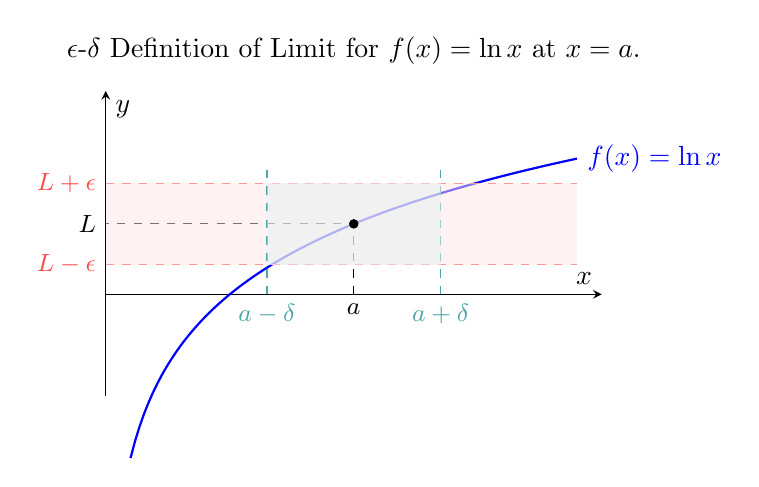
\begin{tikzpicture}
\begin{axis}[
    axis lines=middle,
    xlabel=$x$, ylabel=$y$,
    xmin=0, xmax=4, ymin=-1, ymax=2,
    ticks=none,
    width=0.65\textwidth,
    height=0.45\textwidth,
    clip=false,
    title={$\epsilon$-$\delta$ Definition of Limit for $f(x) = \ln x$ at $x = a$.}
]
    % Curve y = ln(x)
    \addplot[domain=0.2:3.8, samples=100, blue, thick] {ln(x)} node[right] {$f(x) = \ln x$};
    
    % Point a and L
    \def\a{2}
    \def\L{0.693} % ln(2)
    \def\deltaVal{0.7}
    \def\epsVal{0.4}

    % Lines for a and L
    \draw[dashed] (axis cs:\a, 0) -- (axis cs:\a, \L) -- (axis cs:0, \L);
    
    % Epsilon band
    \draw[red!70, dashed] (axis cs:0, \L - \epsVal) node[left, font=\small] {$L - \epsilon$} -- (axis cs:3.8, \L - \epsVal);
    \draw[red!70, dashed] (axis cs:0, \L + \epsVal) node[left, font=\small] {$L + \epsilon$} -- (axis cs:3.8, \L + \epsVal);
    \fill[red!10, opacity=0.5] (axis cs:0, \L - \epsVal) rectangle (axis cs:3.8, \L + \epsVal);

    % Delta band
    \draw[teal!70, dashed] (axis cs:\a - \deltaVal, 0) node[below, font=\small] {$a - \delta$} -- (axis cs:\a - \deltaVal, \L + \epsVal + 0.2);
    \draw[teal!70, dashed] (axis cs:\a + \deltaVal, 0) node[below, font=\small] {$a + \delta$} -- (axis cs:\a + \deltaVal, \L + \epsVal + 0.2);
    \fill[teal!10, opacity=0.5] (axis cs:\a - \deltaVal, \L - \epsVal) rectangle (axis cs:\a + \deltaVal, \L + \epsVal);

    % Points
    \node[below, font=\small] at (axis cs:\a, 0) {$a$};
    \node[left, font=\small] at (axis cs:0, \L) {$L$};
    \filldraw[black] (axis cs:\a, \L) circle (1.5pt);
\end{axis}
\end{tikzpicture}
\end{figure}


Now consider the case of functions of two variables. We say that the limit of a function $f(x, y)$ exists such that
\begin{align*}
\lim_{(x, y) \to (a, b)}{f(x, y)} = L &\iff \forall \epsilon > 0, \exists \delta > 0 \text{ such that } 0 < \sqrt{(x - a)^2 + (y - b)^2} < \delta \\
&\implies |f(x, y) - L| < \epsilon
\end{align*}

Similarly, we can visualize the $\epsilon$-$\delta$ definition of a limit for a two-variable function $f(x, y)$.

% --- 2D Epsilon-Delta Limit Plot in 3D Space (Correct Horizontal Projection to Z-Axis) ---
\begin{figure}[htbp]
\centering
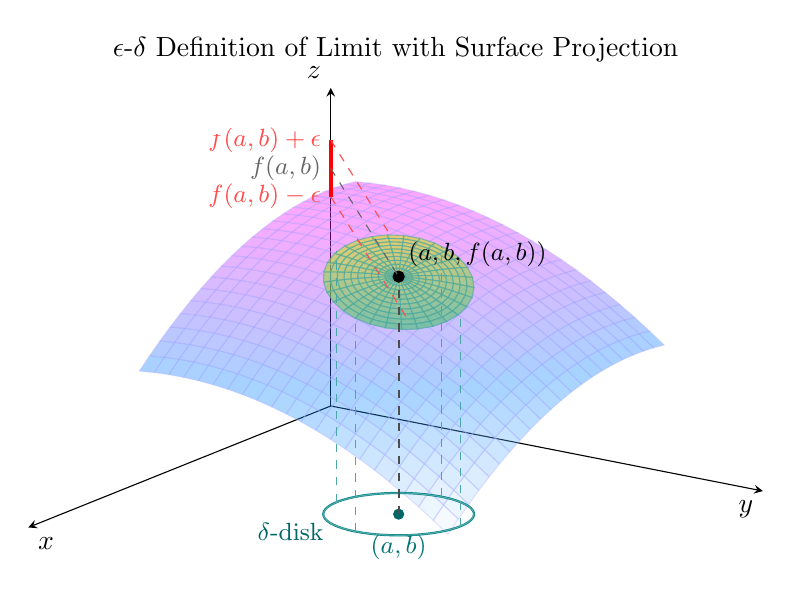
\begin{tikzpicture}
\begin{axis}[
    view={125}{25},
    axis lines=center,
    xlabel=$x$, ylabel=$y$, zlabel=$z$,
    xlabel style={anchor=north west},
    ylabel style={anchor=north east},
    zlabel style={anchor=south east},
    xmin=0, xmax=4.2, ymin=0, ymax=4.2, zmin=0, zmax=4.5,
    ticks=none,
    width=0.9\textwidth,
    height=0.68\textwidth,
    title={$\epsilon$-$\delta$ Definition of Limit with Surface Projection}
]
    % z = f(x,y)
    \addplot3[
        surf, domain=0.8:3.8, domain y=0.8:3.8, samples=22, samples y=22,
        colormap/cool, opacity=0.35, faceted color=blue!30
    ] {3.8 - 0.22*(x-1.2)^2 - 0.22*(y-1.2)^2};

    \def\a{2.2}
    \def\b{2.2}
    \def\L{3.36} % f(2.2, 2.2) = 3.36
    \def\deltaR{0.6}
    \def\eps{0.4}

    % delta disk in xy-plane
    \addplot3[teal, thick, domain=0:360, samples=60] 
        ({\a + \deltaR*cos(x)}, {\b + \deltaR*sin(x)}, {0});
    \addplot3[teal!20, opacity=0.4, domain=0:360, samples=30] 
        ({\a + \deltaR*cos(x)}, {\b + \deltaR*sin(x)}, {0});

    % projection of delta disk onto surface
    \addplot3[
        surf, domain=0:\deltaR, domain y=0:360, samples=12, samples y=30,
        colormap/viridis, opacity=0.6, faceted color=teal!70
    ] ({\a + x*cos(y)}, {\b + x*sin(y)}, {3.8 - 0.22*(\a + x*cos(y) - 1.2)^2 - 0.22*(\b + x*sin(y) - 1.2)^2});

    \pgfplotsinvokeforeach{0, 90, 180, 270}{
        \draw[teal!70, dashed] (axis cs:{\a + \deltaR*cos(#1)}, {\b + \deltaR*sin(#1)}, 0) 
            -- (axis cs:{\a + \deltaR*cos(#1)}, {\b + \deltaR*sin(#1)}, {3.8 - 0.22*(\a + \deltaR*cos(#1) - 1.2)^2 - 0.22*(\b + \deltaR*sin(#1) - 1.2)^2});
    }

   
    \filldraw[teal!80!black] (axis cs:\a, \b, 0) circle (1.8pt);
    \node[teal!90!black, font=\small, below=4pt] at (axis cs:\a, \b, 0) {$(a,b)$};
    \node[teal!80!black, font=\small, left=8pt] at (axis cs:\a+\deltaR, \b, 0) {$\delta$-disk};

    \draw[dashed, black!70, thick] (axis cs:\a, \b, 0) -- (axis cs:\a, \b, \L);

    \filldraw[black] (axis cs:\a, \b, \L) circle (2pt);
    \node[above right, font=\small] at (axis cs:\a, \b, \L) {$(a, b, f(a,b))$};

    \draw[red, ultra thick] (axis cs:0, 0, \L - \eps) -- (axis cs:0, 0, \L + \eps);
    
    \draw[black!60, dashed] (axis cs:0, 0, \L) node[left, font=\small] {$f(a,b)$} -- (axis cs:\a, \b, \L);
    
    \draw[red!70, dashed] (axis cs:0, 0, \L + \eps) node[left, font=\small] {$f(a,b) + \epsilon$} -- (axis cs:\a - 0.35, \b - 0.35, \L + \eps);
    
    \draw[red!70, dashed] (axis cs:0, 0, \L - \eps) node[left, font=\small] {$f(a,b) - \epsilon$} -- (axis cs:\a + 0.35, \b + 0.35, \L - \eps);

\end{axis}
\end{tikzpicture}
\caption{Visualization of the $\delta$-disk in the $xy$-plane and its projection onto the surface $z = f(x,y)$, mapped horizontally to $f(a,b) \pm \epsilon$ on the $z$-axis.}
\end{figure}

\begin{problem}{Limit of a Function of Two Variables}{limit_of_a_function_of_two_variables}
Find, if it exists, $\lim_{(x, y) \to (0, 0)}{\dfrac{xy}{x^2 + y^2}}$.
\end{problem}

\begin{sol}
First, we consider approaching $(0, 0)$ along the $x$-axis, i.e., $y = 0$:
\[
\lim_{x \to 0}{\frac{x(0)}{x^2 + 0^2}} = 0
\]

Next, we consider approaching $(0, 0)$ along the $y$-axis, i.e., $x = 0$:
\[
\lim_{y \to 0}{\frac{0(y)}{0^2 + y^2}} = 0
\]

Next, we consider approaching $(0, 0)$ along the line $y = x$:
\[
\lim_{x \to 0}{\frac{x(x)}{x^2 + x^2}} = \lim_{x \to 0}{\frac{x^2}{2x^2}} = \lim_{x \to 0}{\frac{1}{2}} = \frac{1}{2}
\]

Since approaching along different paths yields different limiting values, the limit does not exist.

\paragraph{Systematic Path Approaches} Checking paths individually can be cumbersome. Instead, we can systematically analyze general path families:

1. Linear Paths ($y = mx$):
   \[
   \lim_{x \to 0}{f(x, mx)} = \lim_{x \to 0}{\frac{x(mx)}{x^2 + (mx)^2}} = \lim_{x \to 0}{\frac{mx^2}{x^2(1 + m^2)}} = \frac{m}{1 + m^2}
   \]
   The limit depends explicitly on the slope $m$. Hence, the limit does not exist.

2. Polar Coordinates ($x = r\cos\theta, y = r\sin\theta$):
   \[
   \lim_{r \to 0}{f(r \cos \theta, r \sin \theta)} = \lim_{r \to 0}{\dfrac{r^2 \cos\theta\sin\theta}{r^2}} = \cos\theta\sin\theta
   \]
   The limit depends on the angle $\theta$, confirming the limit does not exist.
\end{sol}

\begin{definition}{Squeeze Theorem for Two Variables}{squeeze_theorem_for_two_variables}
If $g(x, y) \leq f(x, y) \leq h(x, y)$ for all $(x, y)$ in a disk centered at $(a, b)$ (except possibly at $(a, b)$ itself), and 
\[
\lim_{(x, y) \to (a, b)} g(x, y) = \lim_{(x, y) \to (a, b)} h(x, y) = L
\]
then $\lim_{(x, y) \to (a, b)} f(x, y) = L$.
\end{definition}

\begin{definition}{Continuity of Functions of Several Variables}{continuity_of_functions_of_several_variables}
A function $f(x, y)$ is \textit{continuous} at $(a, b)$ if:
\[
\lim_{(x, y) \to (a, b)} f(x, y) = f(a, b)
\]
Furthermore, $f(x, y)$ is continuous on a domain $D$ if it is continuous at every point $(a, b) \in D$.
\end{definition}

\begin{example}[Continuity of a Composite Function]
Consider $f(x,y) = \arctan\left(\dfrac{y}{x}\right)$. 

The inner function $g(x,y) = \dfrac{y}{x}$ is continuous everywhere except on the line $x = 0$. Since $h(t) = \arctan(t)$ is continuous on $\mathbb{R}$, the composite function $f(x,y) = h(g(x,y))$ is continuous at all points $(x,y) \in \mathbb{R}^2$ where $x \neq 0$.
\end{example}